\heading{理论力学-25春-期末1}

\begin{question}[转动竖直轴上的匀质杆]
一根长为 $l$、质量为 $m$ 的匀质细杆，一端通过光滑铰链与一根绕自身以匀角速度 $\Omega$ 转动的竖直轴相连。讨论时需考虑重力作用。

\begin{center}
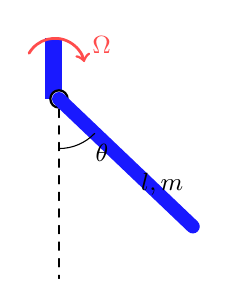
\begin{tikzpicture}[x=1cm,y=1cm,line cap=round,line join=round,font=\small]
  \fill[blue!90] (-0.18,1.18) rectangle (0.04,1.96);
  \draw[line width=0.8pt,fill=white] (0,1.18) circle (0.11);
  \draw[dashed] (0,1.05) -- (0,-1.10);
  \coordinate (P) at (0,1.18);
  \coordinate (Q) at (1.70,-0.44);
  \draw[line width=5pt,blue!90] (P) -- (Q);
  \draw[->,line width=1.0pt,red!70] (-0.38,1.76) arc[start angle=150,end angle=12,radius=0.38];
  \node[red!70,right] at (0.30,1.86) {$\Omega$};
  \draw (0,0.55) arc[start angle=-90,end angle=-44,radius=0.63];
  \node[right] at (0.34,0.50) {$\theta$};
  \node[right] at (0.92,0.10) {$l,m$};
\end{tikzpicture}

{\small 题 1 示意图}
\end{center}

\begin{enumerate}
  \item 写出系统的拉格朗日量，并求当 $\theta$ 为广义坐标时的运动微分方程（写成 $\ddot\theta+\cdots=0$ 的形式）；
  \item 求 $\theta$ 为小量时的解，并讨论其稳定性。
\end{enumerate}

\begin{solution}
设细杆与竖直向下方向的夹角为 $\theta$。杆绕铰链的转动惯量为
\[
  I=\frac13ml^2.
\]
系统动能包括 $\theta$ 方向转动和随竖直轴转动两部分：
\[
  T=\frac16ml^2\dot\theta^2+\frac16ml^2\Omega^2\sin^2\theta.
\]
势能为
\[
  V=-\frac12mgl\cos\theta.
\]
\begin{enumerate}
  \item 拉格朗日量为
  \[
    L=\frac16ml^2\dot\theta^2+\frac16ml^2\Omega^2\sin^2\theta
    +\frac12mgl\cos\theta.
  \]
  拉格朗日方程给出
  \[
    \boxed{\ddot\theta+
    \left(\frac{3g}{2l}-\Omega^2\cos\theta\right)\sin\theta=0}.
  \]
  \item 小角度下
  \[
    \ddot\theta+\left(\frac{3g}{2l}-\Omega^2\right)\theta=0.
  \]
  因此当
  \[
    \boxed{\Omega^2<\frac{3g}{2l}}
  \]
  时，$\theta=0$ 稳定，解为
  \[
    \theta=A\cos\left(\sqrt{\frac{3g}{2l}-\Omega^2}\,t\right)
    +B\sin\left(\sqrt{\frac{3g}{2l}-\Omega^2}\,t\right).
  \]
  当 $\Omega^2>3g/(2l)$ 时，$\theta=0$ 不稳定，并出现倾斜平衡
  \[
    \cos\theta_0=\frac{3g}{2l\Omega^2}.
  \]
\end{enumerate}


\medskip
\textbf{稳定性判断：}等效势可写为
\[
  V_{\mathrm{eff}}(\theta)=-\frac12mgl\cos\theta-\frac16ml^2\Omega^2\sin^2\theta.
\]
平衡位置满足
\[
  \frac{\partial V_{\mathrm{eff}}}{\partial\theta}=0
  \quad\Longleftrightarrow\quad
  \sin\theta\left(\frac12mgl-\frac13ml^2\Omega^2\cos\theta\right)=0.
\]
因此除了 $\theta=0,\pi$ 外，快速转动时还存在倾斜平衡。判断稳定性时应考察 $V_{\mathrm{eff}}''$，而不仅是运动方程的一阶线性化；这可避免把快速转动情形的稳定分支漏掉。
\end{solution}
\end{question}

\begin{question}[转动圆环中的质点]
用哈密顿方法求解下题。如图，空心圆环可绕竖直轴 $AC$ 转动，转动惯量为 $I$。圆环的内壁光滑，半径为 $R$，初始角速度大小为 $\omega_0$。质量为 $m$ 的质点初始时静止在圆环内的 $A$ 点，并在微小扰动后沿环向下滑动。

\begin{center}
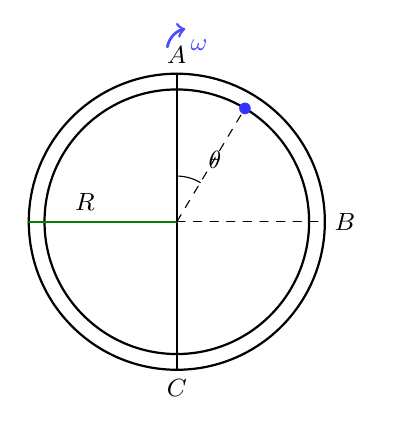
\begin{tikzpicture}[x=1cm,y=1cm,line cap=round,line join=round,font=\small]
  \draw[line width=0.8pt] (0,0) circle (1.88);
  \draw[line width=0.8pt] (0,0) circle (1.68);
  \draw[line width=0.8pt] (0,1.88) -- (0,-1.88);
  \draw[dashed] (0,0) -- (1.88,0);
  \draw[line width=0.8pt,green!50!black] (-1.88,0) -- (0,0);
  \coordinate (A) at (0,1.88);
  \coordinate (B) at (1.88,0);
  \coordinate (C) at (0,-1.88);
  \coordinate (M) at ({1.68*sin(31)},{1.68*cos(31)});
  \fill[blue!80] (M) circle (2.1pt);
  \draw[dashed] (0,0) -- (M);
  \node[above] at (A) {$A$};
  \node[right] at (B) {$B$};
  \node[below] at (C) {$C$};
  \node[above left] at (-0.92,0.02) {$R$};
  \draw (0,0.58) arc[start angle=90,end angle=59,radius=0.58];
  \node[right] at (0.28,0.78) {$\theta$};
  \draw[->,line width=1.0pt,blue!70] (-0.12,2.22) arc[start angle=170,end angle=100,radius=0.28];
  \node[blue!70,right] at (0.05,2.24) {$\omega$};
\end{tikzpicture}

{\small 题 2 示意图}
\end{center}

\begin{enumerate}
  \item 写出系统的哈密顿正则方程；
  \item 写出系统的初积分，并分别求质点滑到 $B$ 点和 $C$ 点时圆环的角速度大小以及质点的速度大小。
\end{enumerate}

\begin{solution}
取质点相对竖直向上方向的夹角为 $\theta$，圆环绕竖直轴的转角为 $\varphi$。质点到转轴的距离为 $R\sin\theta$，故
\[
  T=\frac12mR^2\dot\theta^2
  +\frac12\left(I+mR^2\sin^2\theta\right)\dot\varphi^2,
  \qquad
  V=mgR\cos\theta .
\]
正则动量为
\[
  p_\theta=mR^2\dot\theta,
  \qquad
  p_\varphi=\left(I+mR^2\sin^2\theta\right)\dot\varphi .
\]
\begin{enumerate}
  \item 哈密顿量为
  \ansmath{H=\frac{p_\theta^2}{2mR^2}
    +\frac{p_\varphi^2}{2\left(I+mR^2\sin^2\theta\right)}+mgR\cos\theta.}
  哈密顿正则方程为
  \[
    \dot\theta=\frac{p_\theta}{mR^2},
    \qquad
    \dot\varphi=\frac{p_\varphi}{I+mR^2\sin^2\theta},
  \]
  \[
    \dot p_\theta=\frac{p_\varphi^2mR^2\sin\theta\cos\theta}
    {(I+mR^2\sin^2\theta)^2}+mgR\sin\theta,
    \qquad
    \dot p_\varphi=0 .
  \]
  \item 两个初积分是
  \ansmath{p_\varphi=\text{const.},\qquad H=\text{const.}}
  初始条件为 $\theta=0$、$\dot\theta=0$、$\dot\varphi=\omega_0$，所以
  \[
    p_\varphi=I\omega_0,
    \qquad
    H=\frac12I\omega_0^2+mgR .
  \]
  到达侧点 $B$ 时 $\theta=\pi/2$，有
  \ansmath{\dot\varphi_B=\frac{I\omega_0}{I+mR^2}.}
  沿圆环切向的相对速度 $u_B=R|\dot\theta_B|$ 满足
  \[
    \frac12m u_B^2
    =mgR+\frac12I\omega_0^2-\frac12\frac{I^2\omega_0^2}{I+mR^2},
  \]
  即
  \ansmath{u_B=\sqrt{2gR+\frac{IR^2\omega_0^2}{I+mR^2}}.}
  质点在惯性系中的总速度还包含绕竖直轴的分量 $R\dot\varphi_B$，因此
  \[
    v_{B,\mathrm{inertial}}^2
    =u_B^2+R^2\dot\varphi_B^2 .
  \]
  到达最低点 $C$ 时 $\theta=\pi$，质点到转轴距离为零，因此
  \ansmath{\dot\varphi_C=\omega_0,\qquad u_C=v_{C,\mathrm{inertial}}=2\sqrt{gR}.}
\end{enumerate}
\end{solution}

\end{question}

\begin{question}[旋转矩形薄板的轴承受力]
如图，一块均质矩形薄板的质量为 $m$，边长分别为 $a$ 和 $2a$。以薄板质心为原点建立 $x$--$y$--$z$ 坐标系。薄板绕其对角线以角速度 $\Omega$ 作匀速转动，如图（a）所示。

\begin{center}
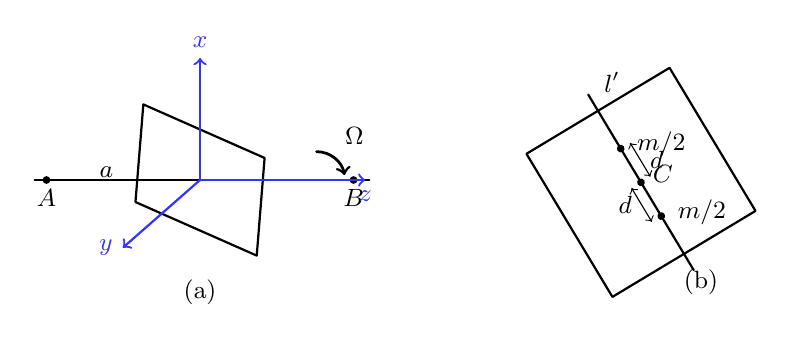
\begin{tikzpicture}[x=1cm,y=1cm,line cap=round,line join=round,font=\small]
  \begin{scope}[shift={(-3.25,0.05)}]
    \coordinate (A) at (-1.95,0);
    \coordinate (B) at (1.95,0);
    \draw[line width=0.8pt] (-2.10,0) -- (2.15,0);
    \fill (A) circle (1.4pt); \fill (B) circle (1.4pt);
    \node[below] at (A) {$A$};
    \node[below] at (B) {$B$};
    \draw[line width=0.8pt] (-0.72,0.96)--(0.82,0.28)--(0.72,-0.96)--(-0.82,-0.28)--cycle;
    \draw[->,blue!80,line width=0.8pt] (0,0) -- (0,1.55) node[above] {$x$};
    \draw[->,blue!80,line width=0.8pt] (0,0) -- (-0.98,-0.86) node[left] {$y$};
    \draw[->,blue!80,line width=0.8pt] (0,0) -- (2.10,0) node[below] {$z$};
    \node[left] at (-0.98,0.10) {$a$};
    \draw[->,line width=1.0pt] (1.48,0.36) arc[start angle=90,end angle=10,radius=0.36];
    \node[right] at (1.72,0.56) {$\Omega$};
    \node at (0,-1.42) {(a)};
  \end{scope}
  \begin{scope}[shift={(2.35,0.02)},rotate=31]
    \draw[line width=0.8pt] (-1.06,-1.06) rectangle (1.06,1.06);
    \draw[line width=0.8pt] (0,-1.30) -- (0,1.30);
    \fill (0,0) circle (1.4pt);
    \node[right] at (0.08,0.08) {$C$};
    \fill (0,0.50) circle (1.4pt);
    \fill (0,-0.50) circle (1.4pt);
    \node[right] at (0.10,0.50) {$m/2$};
    \node[right] at (0.10,-0.50) {$m/2$};
    \node[above right] at (0.02,1.18) {$l'$};
    \draw[<->] (0.14,0) -- (0.14,0.50);
    \node[right] at (0.14,0.25) {$d$};
    \draw[<->] (-0.14,0) -- (-0.14,-0.50);
    \node[left] at (-0.14,-0.25) {$d$};
    \node at (0,-1.48) {(b)};
  \end{scope}
\end{tikzpicture}

{\small 题 3 示意图}
\end{center}

\begin{enumerate}
  \item 求两个轴承处的受力 $N^{(A)}$ 和 $N^{(B)}$（设其 $z$ 分量均为 $0$）；
  \item 若按图（b）所示，在过质心 $C$ 的 $l'$ 轴上焊接两个质量均为 $m/2$ 的质点，以消除转动时产生的轴承受力，求质点到质心的距离 $d$。
\end{enumerate}

\begin{solution}
取 $z$ 轴沿薄板对角线，即转轴方向；取 $x$ 轴在薄板平面内并垂直于 $z$ 轴，$y$ 轴垂直于薄板。设矩形两边方向为主轴 $u,v$，边长分别为 $2a,a$，则
\[
  I_u=\frac1{12}ma^2,
  \qquad
  I_v=\frac1{12}m(2a)^2=\frac13ma^2.
\]
对角线方向为
\[
  \boldsymbol e_z=\frac{2}{\sqrt5}\boldsymbol e_u+\frac1{\sqrt5}\boldsymbol e_v,
\]
在板面内垂直于它的方向为
\[
  \boldsymbol e_x=-\frac1{\sqrt5}\boldsymbol e_u+\frac2{\sqrt5}\boldsymbol e_v.
\]
角速度为 $\boldsymbol\Omega=\Omega\boldsymbol e_z$。角动量在 $x$ 方向的分量为
\[
  L_x=\Omega\frac{2}{5}(I_v-I_u)=\frac1{10}ma^2\Omega.
\]
由于刚体绕 $z$ 轴匀速转动，所需力矩为
\[
  \boldsymbol M=\boldsymbol\Omega\times\boldsymbol L
  =\frac1{10}ma^2\Omega^2\boldsymbol e_y.
\]
\begin{enumerate}
  \item 设两个轴承到质心的距离为
  \[
    c=\frac{\sqrt5}{2}a.
  \]
  质心不动，故两个轴承的横向力满足
  \[
    \boldsymbol N^{(A)}+\boldsymbol N^{(B)}=0.
  \]
  又因题设 $z$ 分量为零，令
  \[
    \boldsymbol N^{(A)}=N_x\boldsymbol e_x,
    \qquad
    \boldsymbol N^{(B)}=-N_x\boldsymbol e_x.
  \]
  由力偶矩
  \[
    -2cN_x\boldsymbol e_y=\frac1{10}ma^2\Omega^2\boldsymbol e_y
  \]
  得
  \[
    \boxed{\boldsymbol N^{(A)}=-\frac{ma\Omega^2}{10\sqrt5}\boldsymbol e_x,
    \qquad
    \boldsymbol N^{(B)}=\frac{ma\Omega^2}{10\sqrt5}\boldsymbol e_x}.
  \]
  若采用相反的 $x$ 轴方向，二者符号同时改变。
  \item 消除轴承受力的条件是使转轴成为整体的主惯量轴，即使惯量积 $I_{xz}$ 为零。原薄板给出
  \[
    I_{xz}=\frac1{10}ma^2.
  \]
  若两个质量为 $m/2$ 的质点对称焊接在过质心的直线 $l'$ 上，且该直线与 $z$ 轴夹角为 $\beta$，则附加惯量积为
  \[
    I_{xz}^{\mathrm{add}}=-md^2\sin\beta\cos\beta.
  \]
  因而
  \[
    d^2=\frac{a^2}{10\sin\beta\cos\beta}
  \]
  （取能使符号相消的方向）。若图中 $l'$ 为矩形另一条对角线，则
  \[
    \sin\beta=\frac45,
    \qquad
    \cos\beta=\frac35,
  \]
  于是
  \[
    \boxed{d=a\sqrt{\frac5{24}}}.
  \]
\end{enumerate}
\end{solution}
\end{question}

\begin{question}[拉格朗日力学与哈密顿力学]
比较拉格朗日力学 $L(q,\dot q,t)$ 与哈密顿力学 $H(q,p,t)$ 的异同。可从自由度、待求量、基本微分方程等角度展开，并讨论二者在推广到非传统力学问题（如量子体系、场论等）时的优缺点。

\begin{solution}
拉格朗日力学与哈密顿力学描述的是同一经典力学体系，但变量和方程形式不同。

拉格朗日力学以广义坐标和广义速度为基本变量：
\[
  L=L(q,\dot q,t).
\]
若系统有 $n$ 个自由度，待求量为 $q_1,\dots,q_n$，基本方程为 $n$ 个二阶微分方程
\[
  \frac{\dd}{\dd t}\frac{\partial L}{\partial\dot q_i}
  -\frac{\partial L}{\partial q_i}=0.
\]
它的优点是便于处理约束、选取广义坐标，并且直接来自变分原理。

哈密顿力学以广义坐标和正则动量为基本变量：
\[
  H=H(q,p,t),
  \qquad
  p_i=\frac{\partial L}{\partial\dot q_i}.
\]
若系统有 $n$ 个自由度，待求量为 $2n$ 个变量 $q_i,p_i$，基本方程为 $2n$ 个一阶方程
\[
  \dot q_i=\frac{\partial H}{\partial p_i},
  \qquad
  \dot p_i=-\frac{\partial H}{\partial q_i}.
\]
它的优点是相空间结构清晰，正则变换、泊松括号、可积系统和统计力学都可自然表述。

在推广方面，拉格朗日形式更适合场论和相对论协变表述，因为作用量
\[
  S=\int L\,\dd t
\]
或
\[
  S=\int\mathcal L\,\dd^4x
\]
可以直接推广。哈密顿形式则更适合量子化，因为正则变量与泊松括号可对应到算符和对易关系。二者互补：拉格朗日形式强调对称性和作用量，哈密顿形式强调相空间和正则结构。


\medskip
\textbf{进一步比较：}若 Legendre 变换非奇异，即矩阵
\[
  \frac{\partial^2L}{\partial\dot q_i\partial\dot q_j}
\]
可逆，则两种表述等价；否则会出现约束哈密顿系统，需要 Dirac 约束理论处理。Lagrange 表述中约束可以较自然地通过广义坐标或乘子进入；Hamilton 表述中约束表现为相空间中的约束面。量子化时 Hamilton 形式常从
\[
  \{q_i,p_j\}=\delta_{ij}
\]
过渡到对易关系，而场论中常从作用量和拉氏密度出发以保持对称性清晰。
\end{solution}
\end{question}

\begin{question}[场论的 Euler--Lagrange 方程]
拉氏密度写作 $\mathcal{L}(\eta_\alpha,\eta_{\alpha,\mu},x_\mu)$，其中 $\eta_\alpha$（$\alpha=1,2,\dots,n$）是彼此独立的场变量。
\begin{enumerate}
  \item 用哈密顿原理推导 Euler--Lagrange 方程，要求给出详细步骤；
  \item 取 $x_\mu=(x,y,z,\ii t)$，并令光速 $c=1$。若拉氏密度为
  \[
    \mathcal{L}=-\phi_{,\mu}\phi^*_{,\mu}-m^2\phi\phi^*+\lambda(\phi\phi^*)^2,
  \]
  利用（1）中得到的 Euler--Lagrange 方程，分别求独立场量 $\phi$ 与 $\phi^*$ 所满足的运动方程。
\end{enumerate}

\begin{solution}
\begin{enumerate}
  \item 作用量为
  \[
    S=\int \mathcal L(\eta_\alpha,\eta_{\alpha,\mu},x_\mu)\,\dd^4x.
  \]
  对独立场量 $\eta_\alpha$ 作变分，且令边界变分为零：
  \[
    \delta S=\int\left(
    \frac{\partial\mathcal L}{\partial\eta_\alpha}\delta\eta_\alpha
    +\frac{\partial\mathcal L}{\partial\eta_{\alpha,\mu}}
    \delta\eta_{\alpha,\mu}
    \right)\dd^4x.
  \]
  由于
  \[
    \delta\eta_{\alpha,\mu}=\partial_\mu\delta\eta_\alpha,
  \]
  分部积分并忽略边界项得
  \[
    \delta S=\int\left[
    \frac{\partial\mathcal L}{\partial\eta_\alpha}
    -\partial_\mu\left(
    \frac{\partial\mathcal L}{\partial\eta_{\alpha,\mu}}
    \right)
    \right]\delta\eta_\alpha\,\dd^4x.
  \]
  因 $\delta\eta_\alpha$ 任意，得到场的 Euler--Lagrange 方程
  \[
    \boxed{\frac{\partial\mathcal L}{\partial\eta_\alpha}
    -\partial_\mu\left(
    \frac{\partial\mathcal L}{\partial\eta_{\alpha,\mu}}
    \right)=0}.
  \]
  \item 对
  \[
    \mathcal{L}=-\phi_{,\mu}\phi^*_{,\mu}-m^2\phi\phi^*+
    \lambda(\phi\phi^*)^2
  \]
  分别把 $\phi$ 和 $\phi^*$ 看成独立场量。对 $\phi^*$ 变分：
  \[
    \frac{\partial\mathcal L}{\partial\phi^*}
    =-m^2\phi+2\lambda(\phi\phi^*)\phi,
    \qquad
    \frac{\partial\mathcal L}{\partial\phi^*_{,\mu}}=-\phi_{,\mu}.
  \]
  故
  \[
    \boxed{\phi_{,\mu\mu}-m^2\phi+2\lambda(\phi\phi^*)\phi=0}.
  \]
  同理
  \[
    \boxed{\phi^*_{,\mu\mu}-m^2\phi^*+2\lambda(\phi\phi^*)\phi^*=0}.
  \]
\end{enumerate}
\end{solution}
\end{question}

\begin{question}[阻尼振子与 Hamilton--Jacobi 方程]
设 $\lambda,\omega,m$ 均为正实数，单自由度系统的拉格朗日量为
\[
  L(q,\dot q,t)=\ee^{\lambda t/m}\left(\frac12m\dot q^2-\frac12m\omega^2q^2\right).
\]
对相应的哈密顿量施加由第二类生成函数
\[
  F_2(q,P,t)=\ee^{\lambda t/(2m)}qP
\]
给出的正则变换。
\begin{enumerate}
  \item 求变换后的哈密顿量 $K(Q,P,t)$；
  \item 在新的正则变量 $Q,P$ 下，利用 Hamilton--Jacobi 方程求系统的运动解（积分可以保留为积分形式）；
  \item 讨论不同参数 $\lambda,\omega,m$ 取值时原问题 $q(t)$ 的三类解，并写出 $q(t)$ 的具体形式。
\end{enumerate}

提示：本题中可能用到如下积分公式（$A_1,B_1>0$）：
\[
  \int\frac{\dd x}{\sqrt{B_1-A_1x^2}}
  =\frac{1}{\sqrt{A_1}}\arcsin\left(\sqrt{\frac{A_1}{B_1}}x\right)+C_1,
\]
\[
  \int\frac{\dd x}{\sqrt{B_1+A_1x^2}}
  =\frac{1}{\sqrt{A_1}}\operatorname{arcsinh}\left(\sqrt{\frac{A_1}{B_1}}x\right)+C_2,
\]
其中 $C_1$、$C_2$ 为任意积分常数。

\begin{solution}
正则动量为
\[
  p=\frac{\partial L}{\partial\dot q}=m\ee^{\lambda t/m}\dot q,
  \qquad
  \dot q=\frac{p}{m}\ee^{-\lambda t/m}.
\]
因此原哈密顿量为
\[
  H(q,p,t)=p\dot q-L
  =\frac{p^2}{2m}\ee^{-\lambda t/m}
  +\frac12m\omega^2q^2\ee^{\lambda t/m}.
\]
由第二类生成函数
\[
  F_2(q,P,t)=\ee^{\lambda t/(2m)}qP
\]
得
\[
  Q=\frac{\partial F_2}{\partial P}=\ee^{\lambda t/(2m)}q,
  \qquad
  p=\frac{\partial F_2}{\partial q}=\ee^{\lambda t/(2m)}P.
\]
新哈密顿量为
\[
  K=H+\frac{\partial F_2}{\partial t}
  =\frac{P^2}{2m}+\frac12m\omega^2Q^2+\frac{\lambda}{2m}QP.
\]
配方可写为
\[
  K=\frac{1}{2m}\left(P+\frac\lambda2Q\right)^2
  +\frac12m\left(\omega^2-\frac{\lambda^2}{4m^2}\right)Q^2.
\]
令
\[
  \gamma=\frac{\lambda}{2m},
  \qquad
  \Omega^2=\omega^2-\gamma^2.
\]
Hamilton--Jacobi 方程取分离形式 $S=W(Q,E)-Et$，则
\[
  \frac{1}{2m}\left(\frac{\partial W}{\partial Q}\right)^2
  +\frac{\lambda}{2m}Q\frac{\partial W}{\partial Q}
  +\frac12m\omega^2Q^2=E.
\]
解得
\[
  \frac{\partial W}{\partial Q}
  =-\frac\lambda2Q\pm\sqrt{2mE-m^2\Omega^2Q^2},
\]
从而
\ansmath{S(Q,E,t)=-Et-\frac\lambda4Q^2
  \pm\int^Q\sqrt{2mE-m^2\Omega^2u^2}\,\dd u.}
当 $\Omega^2$ 为正、零、负时，上式中的积分分别化为反正弦型、幂函数型、反双曲正弦型。

原变量 $q$ 直接满足
\[
  \ddot q+\frac{\lambda}{m}\dot q+\omega^2q=0.
\]
因此三类解为：
\begin{enumerate}
  \item 欠阻尼 $\omega^2>\lambda^2/(4m^2)$：
  \ansmath{q(t)=\ee^{-\lambda t/(2m)}
    \left(C_1\cos\Omega t+C_2\sin\Omega t\right),
    \quad
    \Omega=\sqrt{\omega^2-\frac{\lambda^2}{4m^2}}.}
  \item 临界阻尼 $\omega^2=\lambda^2/(4m^2)$：
  \ansmath{q(t)=\ee^{-\lambda t/(2m)}(C_1+C_2t).}
  \item 过阻尼 $\omega^2<\lambda^2/(4m^2)$：令
  \[
    \kappa=\sqrt{\frac{\lambda^2}{4m^2}-\omega^2},
  \]
  则
  \ansmath{q(t)=\ee^{-\lambda t/(2m)}
    \left(C_1\ee^{\kappa t}+C_2\ee^{-\kappa t}\right).}
\end{enumerate}
正则动量由
\[
  p=m\ee^{\lambda t/m}\dot q
\]
求得。
\end{solution}

\end{question}
